\section{Theory-guided Approaches}
\label{sec:tga}
Partial Differential Equations (PDE) has often to be solved in physics. Thus, besides the observational data from experiments, the underlying equations that describes the physics of the process are also known. The approaches that use not only pure data, but also integrate the underlying physics of the process into the machine learning models are called theory-guided~\cite{tgds} or physics-informed~\cite{Raissi19}. 

Theory-guided approaches can be further classified by their source, representation and integration~\cite{inltax}; or more detailed into Basic ML, Physics-Guided
Loss Function, Physics-Guided Initialization, Physics-Guided Architecture, Residual Model and Hybrid Model~\cite{survey}. Other ways to classify the theory-guided PDE Solvers are the applied numeric scheme (finite difference, finite volume or finite element-based) or type of equation (elliptic, parabolic, hyperbolic).

Since in the recent works the diverse combinations from the different categories are applied, we use in the following subsections the classification from Gao et al.~\cite{Gao21} into continuous and discrete.


\subsection{Continuous Approaches}
Continuous physics-informed approaches are a baseline for many physical problems. They commonly employ the fully-connected neural network architecture. Continuous approaches use point-wise automatic differentiation technique~\cite{ad} to compute space and time derivatives and approximate the continuous solution of PDE with respect to given coordinates. 

\subsubsection{Physics-informed Neural Networks (PINNs)}
Similar approaches existed earlier~\cite{similarPINN}, but Raissi et al.~\cite{Raissi19, Raissi1, Raissi2} have first formulated them as a new paradigm --- Physics-Informed Neural Networks (PINNs) --- to solve all types of PDEs. 

Most supervised machine learning approaches require much data and do not take into account physical laws and, thus, usually fail when applied to a limited amount of data. To mitigate this problem, the prior knowledge defined by physical equation induces the loss function of the trained network. This acts as a regularizer and restricts the solution space incorporating the PDE.

Raissi et al.~\cite{Raissi19} investigate two major problems: data-driven solution~\cite{Raissi1} and data-driven discovery~\cite{Raissi2} of PDEs. In these works, they use simple fully-connected (FC) feed-forward networks without additional regularization, and hyperbolic tangent activation function. The method was evaluated on Schrödinger, Allen--Cahn, Korteq--de Vries and Navier--Stokes equations and showed promising results. 

\subsubsection{Diversity of approaches}
The proposed by Raissi et al. method is applied to many scientific areas: nano-optics~\cite{nanooptics}, elastodynamics~\cite{elastodynamics}, diagnosing atrial fibrillation  ~\cite{fibrillation}. Moreover, NVIDIA created a SimNet framework based on continuous physics-informed approaches to assist in solving physics problems on their GPUs~\cite{nvidia}.

Despite the broad application of continuous PINNs, all of them have similar limitations. First, continuous approaches have high computational training costs. Second, integrating of proper initial and boundary condition for more than 2-D spaces in PDE requires hard ad hoc designing~\cite{Gao21}. Therefore, describing constraints for more complicated real-world PDEs remains challenging using continuous approaches. Third, the theoretical error and convergence estimations are absent in the model. Thus, employing Bayesian optimization~\cite{sno12} is a part of the future works.

Finally, the authors point out that the proposed method is not a replacements of exiting numerical methods, but a supplement for hybrid models to enhance the quality and and reduce the computational cost of predictions. Moreover, the questions e.g. about depth and structure of the model, amount of needed data, possibility of vanishing and exploding gradients, etc. remain uninvestigated. 


\subsection{Discrete Approaches}
Discrete physics-informed approaches have reduced computational costs and better scalability compared to continuous ones. They commonly employ convolutional neural network (CNN) architecture. Discrete approaches use automatic differentiation technique~\cite{ad} to learn space and time solutions directly based on numerical discretization scheme.

\subsubsection{Data-driven Discretization}
Typical pipeline for solving PDEs consists of three main steps. First, we take a PDE that simulates a physical process e.g. Burgers equation $\frac{\partial v}{\partial t}+v \frac{\partial v}{\partial x}=\eta \frac{\partial^{2} v}{\partial x^{2}}$. Second, discretize it in space and represent on the mesh e.g. $\quad \frac{\partial^{2} v}{\partial x^{2}} \approx \frac{v_{i+1}-2 v_{i}+v_{i-1}}{\Delta x^{2}}$. This results in a large set of ODEs that can be solved numerically. If we want to understand what happens in simulation e.g. weather simulation, $\Delta x$ must be small, whereby the number of mesh points must be large. 

Numerical solutions of a PDE is difficult. Therefore, applied mathematics tries to derive an effective equation that can be solved numerically with lower computational power. This analytical process is usually ad hoc and difficult~\cite{brennerLecture}. To mitigate it, Bar--Sinai et al.~\cite{Brenner19} propose a Data-driven Discretization method.

All solutions of PDEs are in infinite dimensions, but the solutions for a concrete PDE instance are in low-dimensional manifold~\cite{titi89}. Therefore, the main idea is to parameterize solution manifold and execute machine learning model to obtain it. Hence, for a given PDE:
\begin{equation}
    \begin{array}{l}\frac{\partial v}{\partial t}=\mathcal{L}(t, x, v, \nabla v, \nabla \nabla v, \ldots) \end{array}
    \label{eq:ddd1}
\end{equation}
Discretize in finite differences and approximate with weights and mesh points:
\begin{equation}
    \begin{array}{l}\quad \frac{\partial^{n} v}{\partial x^{n}}|_{x_{i}+\frac{\Delta x}{2}} \approx \sum_{k=-N}^{N} \alpha_{k}^{(n)} \hat{v}_{i+k} \end{array}
    \label{eq:ddd2}
\end{equation}
Classical approaches derive weights from calculus, but in this approach ${\alpha}_{k}^{(n)}$ is learned instead. Intuitively, it helps to learn how the solutions look like based on data, instead of performing direct interpolation. For example, the comparison between polynomial and neural net interpolation is shown in \cref{fig:ddi}.

\begin{figure}
	\centering
	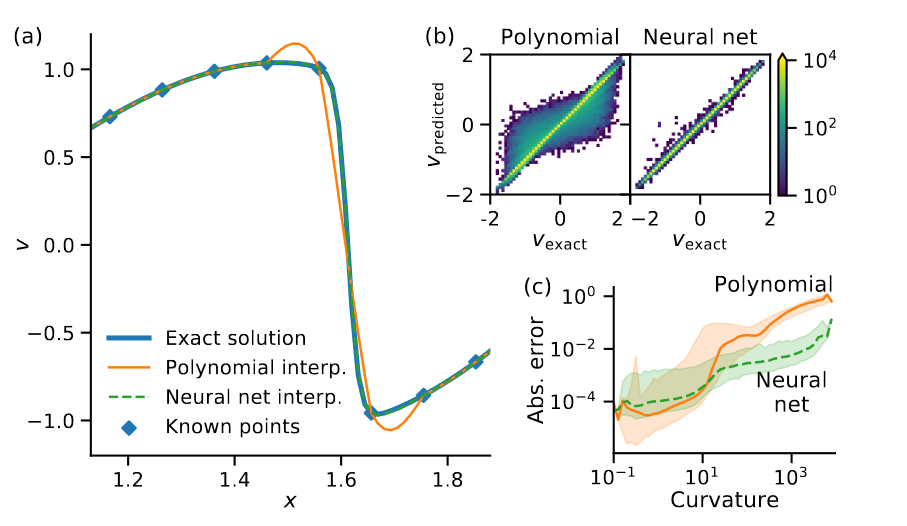
\includegraphics[width=10cm]{figures/ddinterpolation.png}
	\caption{Comparison between polynomial and neural net interpolation. Intuition: instead of performing direct polynomial interpolation, learn the solution manifold based on data, i.e. how the solutions look like~\cite{Brenner19}.}
	\label{fig:ddi}
\end{figure}  

The method Data-driven Discretization consists of three steps: perform many high-resolution simulations, train a regressor algorithm to machine learn the solution manifold and use it to estimate spatial derivatives from low-resolution data and integrate over them.

The method was evaluated on Burgers, Kuramoto--Sivashinsky and Korteweg--de Vries equations. The authors achieved remarkably accurate results for one-dimensional problems with 4-8 times coarser discretization resolution compared to standard finite difference methods.

This approach suffers from two major limitations. First, CNN requires more computational operations than finite difference implementation. This results in problems with inference speed. Second, the method was mainly evaluated in one dimension, while real-world problems have usually two or more dimensions.

To address this issue, Kochkov et al.~\cite{Brenner20} investigate Data-driven Discretization in the following work and adjust it for two-dimensional problems. 

Both training and inference are shown in \cref{fig:ddd}. First steps do not differ from the original Data-driven discretization. The CNN learns to predict finite difference coefficients in the spatial derivatives. Then, finite volume scheme is used to compute time derivatives, as performed in the numerical method of lines~\cite{schiesser91}. In contrast to the previous method, the results are accumulated over 10 timestamps to minimize the difference between model predictions and ground truths from high-resolution simulations. Multi-step mean absolute error (MAE) loss function is employed. Furthermore, in contrast to the previous method, physical constraints are employed before and after neural net. To guarantee stability, normalization of input features is applied. The entire program is written in automatic differentiation framework TensorFlow to enable training a neural net inside the classical numerical solver.

\begin{figure}
	\centering
	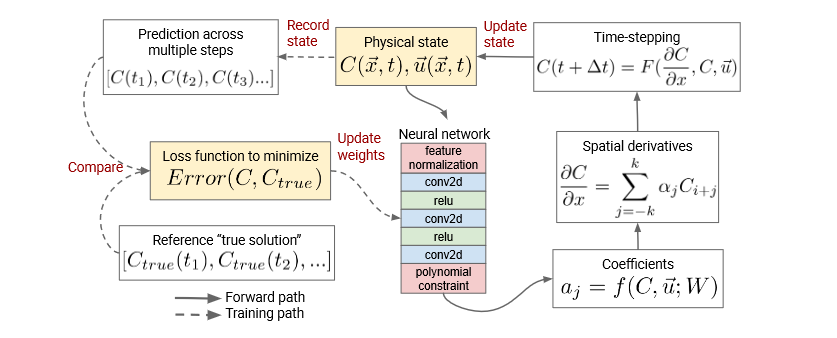
\includegraphics[width=12cm]{figures/ddd.png}
	\caption{Data-driven Discretization Framework~\cite{Brenner20}.}
	\label{fig:ddd}
\end{figure}  

Evaluated on 2-D Advection PDE, the adjusted Data-driven Discretization showed the same accuracy as the state-of-the-art numerical solver by 4 times coarser resolution in all dimensions. However, the model fails when trying to predict for predicting longer time period that it was trained. 

In order to correctly predict for out of training distribution inputs, Kochkov et al.~\cite{Brenner21} present a novel type of machine learning solvers based on Data-driven Discretization. 

The idea is to take classical state-of-the-art numerical solvers: direct numerical simulation (DNS) and large eddy simulation (LES). Replace error-prone parts such as discretization and closure affected by loss of resolution with machine learning alternatives in DNS and LES, respectively. 

Kochkov et al. propose two approaches. Learned Interpolation (LI) that replaces polynomial interpolation without prior knowledge in DES, as shown in the previous works~\cite{Brenner19, Brenner20}. And Learned Correction (LC) that models a residual correction to the discretization in LES. The principle distinction between these methods is shown in \cref{fig:lilc}. LI employs CNN architecture, while LC uses ResNet. 

Both approaches were evaluated on challenging Navier-Stokes Equation in 2D. They do not suffer from the lack of generalization compared to the predecessor. Moreover, they show the same accuracy as baseline solvers with 8-10 times coarser resolution in each dimension and 40-80 times computational speed-up. Thus, the recent approach has solved the problems encountered in the first versions of Data-driven Discretization solvers.

The evolution of the approaches based on Data-driven Discretization show another possibility to embed the physical constraints into PDE solvers. Compared to the classical PINNs, which mainly apply ``soft'' constraints in form of the loss function, these approaches apply ``hard'' constraints. They replace only some components of numerical solvers with neural nets and, hence, can impose the physical constraints before and after machine learning solvers per construction. This type of synergy improves the existing solvers and guarantees physical consistency at the same time.

\begin{figure}
	\centering
	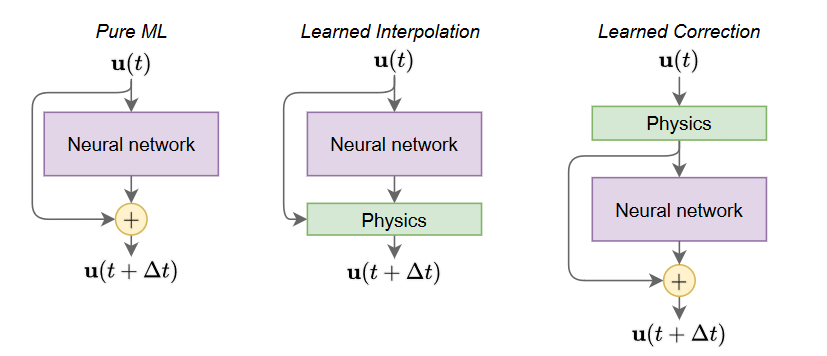
\includegraphics[width=12cm]{figures/lilc.png}
	\caption{The principle difference between Pure ML methods and proposed Learned Interpolation and  Learned Correction is in position of applied physics constraints~\cite{Brenner21}.}
	\label{fig:lilc}
\end{figure}  


\subsubsection{Data-free Discretization}

Data-driven approaches often require large data-sets obtained by high-cost computational simulations on supercomputers. To resolve this problem a series of works investigate the data-free approaches.

These approaches use neural networks to generate data constrained by physical loss in spirit of classical PINNs and iteratively learn to enhance the solutions as performed in numerical solvers.

Ranade et al. propose a DiscretizationNet~\cite{Ranade20}. This ML-Solver comprises a finite volume based discretization scheme in neural network within the automatic differentiable computational graph. Neural network employs a generative encoder-decoder CNN architecture and is shown in \cref{fig:discretizationnet}. Inputs consist from flow variables, boundary condition encoding and geometry encoding. First, the encoder encodes the inputs in lower dimensional latent vector. The latent vector is extended with boundary condition and geometry encoding to enrich the latent space. Second, the latent vector is decoded. Outputs are inserted as inputs into the network again. The iterative process continues until the determined time or reached accuracy. In the training process the physical loss is incorporated in spirit of classical PINNs.

Compared to traditional computational fluid dynamics (CFD) solver ANSYS, the proposed method shows better performance and training stability for three steady Navier--Stokes cases: lid-driven cavity, laminar flow past cylinder and conjugate heat transfer. In future works, the ML-Solver can be investigated for unsteady problems by extending with LSTMs and for other types of PDEs with more complex physics.

\begin{figure}
	\centering
	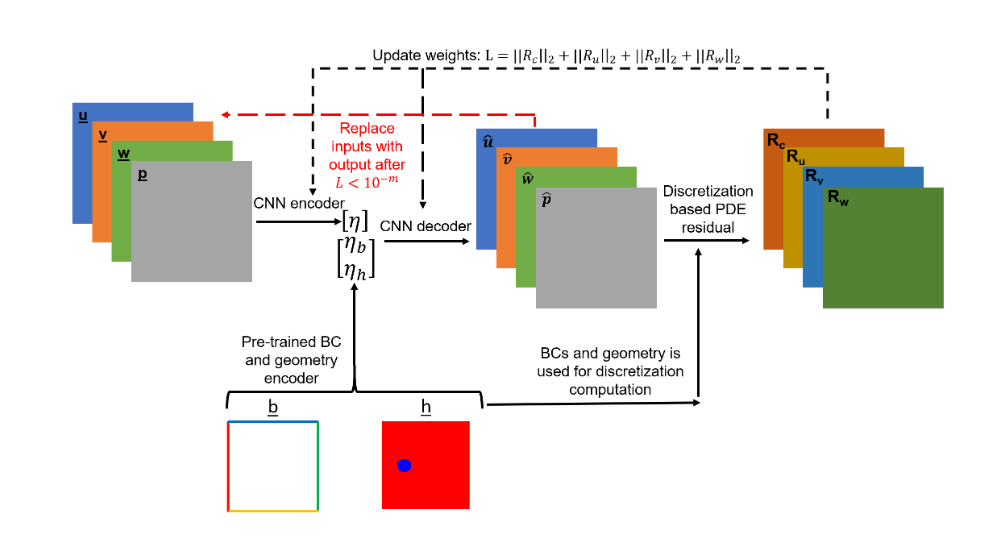
\includegraphics[width=12cm]{figures/discretizationnet.png}
	\caption{Architecture DiscretizationNet for Navier--Stokes Equation. This employs a generative encoder-decoder CNN for data-free PDE learning~\cite{Ranade20}.}
	\label{fig:discretizationnet}
\end{figure}  

\subsubsection{Finite element based Discretization}

The aforementioned works apply finite difference or finite volume schemes. Since the finite element scheme is more accurate for numerous tasks, Yao et al. propose a FEA-Net~\cite{feanet}. This is a discrete PINN based on FEM that employs CNN architecture. The special FE-based convolution is introduced to calculate PDE residuals in physics-informed loss. Due to convolutional backbone the methods are limited to rectangular domains and cannot model irregular geometries with unstructured meshes, so as all CNN-based networks. Since the Fully-connected architecture also suffers from problems such as scalability and incorporation of hard boundary conditions, Gao et al.~\cite{Gao21} propose a novel framework that is based on FEM and employs Graph Convolutional Networks (GCN).

The proposed method has three main features. First, in the input vector of GCN, each spatial coordinate of the mesh has its own node. After forward propagation, GCN outputs the graph with discretized solution fields, where each solution vector is in a separate node. This structure does not require rasterization and allows to internally handle unstructured mesh with simplex quadrilateral elements in spirit of classical FEM solver. Second, Gao et al. apply piece-wise polynomial basis functions that help to make predictions based on output graph. This decreases the search space dimension to improve PDE-informed convergence. Third, the essential boundary conditions are enforced by construction. Therefore, no tuning of penalty coefficient is required. 

Evaluated on Poisson and steady Navier--Stokes problems, the proposed method mitigates the problems caused by FC and CNN architectures and shows the effectiveness and robustness against them. The authors point out the use of combination of deep learning and numerical methods rather than their separation in future works, in order to improve generalability and achieve better results.
